\begin{frame}[noframenumbering,plain]
    \setcounter{framenumber}{1}
    \frametitle{Knowledge Transfer Between Tasks and Languages in the Encoder-agnostic Transformer-based Models}
    Authors: Dmitry Karpov, Vasily Konovalov
    MIPT, Dolgoprudny, Russia
    
\end{frame}



\begin{frame}{Encoder-agnostic models: task}
\begin{enumerate}
    \item Определить закономерности переноса знаний в энкодер-агностичных многозадачных нейросетевых моделях между различными диалоговыми задачами.
    \item Провести оценку зависимости этого переноса от размера обучающей выборки.
 \end{enumerate}
\end{frame}

\begin{frame}{Encoder-agnostic models: architecture}
В 2 словах - отдельный задаче-специфичный линейный слой на каждую задачу, который применяется к выходу энкодера.
Достоинства архитектуры:
\begin{itemize}
  \item Вычислительная и архитектурная простота
  \item Расширяемость на различные типы задач
  \item Не требует псевдоразметки
  \item Можно быстро заменить энкодер
\end{itemize}
The architecture is integrated into the open-source DeepPavlov library.
\end{frame}

\begin{frame}{Encoder-agnostic models: data, sampling}
Принцип подбора данных:
\begin{itemize}
    \item Разговорные задачи
    \item Совпадающие классы для английского и русского языка
\end{itemize}
Сэмплирование примеров на каждом этапе обучения - батч из каждого набора данных с вероятностью пропорционально размеру (plain sampling).
\end{frame}

\begin{frame}{Encoder-agnostic models: данные}
\begin{itemize}
    \item Для классификации \textbf{эмоций} -- русскоязычный набор данных CEDR, собранный из различных интернет-источников, и англоязычный набор данных go\_emotions, собранный из комментариев на ресурсе «Реддит». Использовалось семь типов эмоций по Экману -- ярость, страх, грусть, удовольствие, удивление, отвращение, нейтральная.
    \item Для классификации \textbf{тональности} -- англоязычный набор данных DynaSent(r1), состоящий из предложений, возникающих в диалогах, и русскоязычный набор данных RuReviews, состоящий из отзывов крупного российского электронного магазина. Использовалось три класса -- положительный, отрицательный, нейтральный.
\end{itemize}
\end{frame}

\begin{frame}{Encoder-agnostic models: данные}
\begin{itemize}
    \item Для классификации \textbf{токсичности} -- русскоязычный набор комментариев с ресурса «Двач» (RuToxic) и англоязычный набор комментариев из Википедии (Wiki Talk). Использовалось два класса -- токсичный и не токсичный.
    \item Для классификации \textbf{тем и классификации интентов} -- набор данных MASSIVE, состоящий из обращенных к диалоговой системе фраз пользователей. Набор существует и использовался как в англоязычном, так и в русскоязычном варианте. Каждая фраза из набора принадлежит к одной из 60 тем и к одному из 18 интентов.
\end{itemize}
\end{frame}

\begin{frame}{Encoder-agnostic models: сравнение с однозадачными, английский язык}
\begin{table}[htbp]
\centering
\caption {Метрики англоязычных моделей (точность/макро-F1) для пяти англоязычных диалоговых задач.Режим S означает однозадачные модели, режим M означает многозадачные модели. Усреднено по трем запускам.}
\scalebox{0.7}{
\begin{tabular}{|c|c|c|c|c|c|c|c|}
\hline
\multirow{2}{*}{\textbf{Модель}} & \multirow{2}{*}{\textbf{Режим}} & \multirow{2}{*}{\textbf{Среднее}} & Эмоции & Тональность & Токсичность & Интенты & Темы \\
& & & 39.4k & 80.5k & 127.6k & 11.5k & 11.5k \\ \hline \hline
\textit{\multirow{2}{*}{distilbert}} & S & \textbf{82.9} & \textbf{70.3} & 74.7 & 91.5 & \textbf{87.4} & \textbf{91.0} \\ %\hline
 & M  & 82.1 & 67.7 & \textbf{75.2} & 90.6 & 86.3 & 90.8  \\ \hline
\textit{\multirow{2}{*}{bert}} & S & \textbf{83.9} & \textbf{71.2} & 76.1 & \textbf{93.2} & \textbf{87.9} & \textbf{91.3} \\ %\hline
 & M &  83.0 & 69.0 & \textbf{76.5} & 91.4 & 87.1 & 91.2 \\ \hline
 \end{tabular}}
 \end{table}
 \end{frame}


\begin{frame}{Encoder-agnostic models: сравнение с однозадачными, GLUE}
\begin{table}[htbp]
\caption{Метрики многозадачной энкодер-агностичной модели для набора задач GLUE. M.Corr означает корреляцию Мэттью, P/S означает корреляцию Пирсона-Спирмена, Acc точность, F1 - макро-F1. Режим S означает однозадачные модели, режим M означает многозадачные модели. Размер означает размер тренировочного набора данных.}
%\resizebox{\textwidth}{!}
\scalebox{0.52}{
\begin{tabular}{|c|c|c|c|c|c|c|c|c|c|c|c|}
\hline
\multirow{3}{*}{Модель} & \multirow{3}{*}{Режим}  & Среднее & CoLA & SST-2 & MRPC &STS-B &QQP&MNLI & QNLI & RTE & AX  \\
\cline{3-11}
   &  & Размер  & 8.6k & 67.3k & 2.5k & 5.7k & 363.8k & 392.7k & 104.7k & 2.5k & As MNLI  \\ 
\cline{3-11}   
   &  & метрика  & M.Corr & Acc & F1/Acc & P/S Corr & F1/Acc & Acc (m/mm) & Acc & Acc & M.Corr \\ \hline \hline
Человек & - & 87.1 & 66.4 & 97.8 & 86.3/80.8 & 92.7/92.6 & 59.5/80.4 & 92.0/92.8 & 91.2 & 93.6 & - \\ \hline
\textit{\multirow{2}{*}{distilbert}} & S & 73.3 & \textbf{42.4} & \textbf{92.1} & 85.6/\textbf{80.3} & 78.8/76.8 & \textbf{69.5/88.5} & \textbf{81.3/80.8} & \textbf{87.5} & 52.1 & 29.9  \\ 
 & M & \textbf{74.5} & 36.0 & 91.0 & \textbf{85.7}/79.9 & \textbf{82.6/81.6} & 68.4/87.4 & 80.4/80.3 & 86.0 & \textbf{69.5} & \textbf{30.1} \\  \hline
\textit{\multirow{2}{*}{bert}} & S & 77.3 & \textbf{53.7} & \textbf{93.2} & \textbf{87.7/82.8} & 83.8/82.2 & \textbf{70.3/88.9} & \textbf{83.8/83.1} & \textbf{90.6} & 62.1 & 32.1 \\ 
 & M & \textbf{77.8} & 45.8 & 92.9 & 86.8/82.2 & \textbf{85.3/84.7} & 70.2/88.6 & 83.5/82.6 & 90.1 & \textbf{74.5} & \textbf{32.8} \\  \hline
\end{tabular}}
\end{table}
%\end{table*}
\end{frame}


 
 \begin{frame}{Encoder-agnostic models: сравнение с однозадачными, русский язык}
\begin{table}[htbp]
\centering
\caption {Метрики русскоязычных моделей (точность/f1 macro) для пяти диалоговых задач. Режим S означает однозадачные модели, режим M означает многозадачные модели. Усреднено по трем запускам.} 
\scalebox{0.7}{
\begin{tabular}{|c|c|c|c|c|c|c|c|}
\hline
\multirow{2}{*}{\textbf{Модель}} & \multirow{2}{*}{\textbf{Режим}} & \multirow{2}{*}{\textbf{Среднее}} & Эмоции & Тональность & Токсичность & Интенты & Темы \\
& & & 6.5k & 82.6k & 93.3k & 11.5k & 11.5k \\ \hline \hline
\textit{\multirow{2}{*}{distilrubert}} & S & 86.9 & 82.2 & 77.9 & 97.1 & 86.7 & 90.4  \\
 & M & 86.3 & 81.0 & 77.7 & 96.9 & 85.2 & 90.7 \\ \hline
\textit{\multirow{2}{*}{rubert}} & S & 86.5 & 80.9 & 78.0 & 97.2 & 86.2 & 90.0  \\ 
 & M & 86.2 & 80.5 & 77.6 & 96.8 & 85.3 & 90.5 \\ \hline
 \end{tabular}}
 \end{table}
 

\end{frame}

\begin{frame}{Энкодер-агностичные модели - эффект уменьшения размера выборки, данные на английском языке}
\scalebox{1}{
\begin{minipage}{0.5\textwidth}{
\begin{tikzpicture}
\label{fig:tr-ag:en_dialog_part}
\begin{axis}[xlabel = Процент используемых тренировочных данных,
ylabel = Средняя точность,
legend pos= south east,
% width=10cm,
% height=10cm,
% xmin=2,
% xmax=100,
xtick={2,3,5,7,9,10,15},
ymin=40,ymax=85,
legend cell align={left},
legend style={nodes={scale=0.7, transform shape}}
]
\addplot[color=blue,solid, mark=*] coordinates {
(2, 64.8)%50
(3, 68.8)%50
(5, 71.7)%100
(7,74.2)
%(7.5,74.6)
% (8,74.9)
(9,75.4)
(10, 75.9)%300
(15, 77.4)
};
\addlegendentry{Многозадачные модели}
\addplot[color=green,dashed,mark=*] coordinates {
(2, 44.9)%50
(3, 59.6)%100
(5, 69.1)%300
(7,73.5)
%(7.5,73.5)
% (8,73.8)%500
(9,76.7)
(10,77.1)
(15, 78.5)
};
\addlegendentry{Однозадачные модели}
\end{axis}%
\end{tikzpicture}}
\end{minipage}

\begin{minipage}{0.2\textwidth}
\scalebox{0.7}{
\begin{tabular}[baseline={(0,2.1)}]{|l||c|c|}
\hline
Доля & S & M \\ % Sizes are different for RU and RU+EN, so I don't give them here
\hline \hline
2 & 44.9 & 64.8 \\ \hline
3 & 59.6 & 68.8  \\ \hline
5 & 69.1 & 71.7 \\ \hline
7 & 73.5 & 74.2  \\ \hline
9 & 76.7 & 75.4  \\ \hline
10 & 77.1 & 75.9 \\ \hline
15 & 78.5 & 77.4  \\ \hline
\end{tabular}}
\end{minipage}
}
%
\end{frame}


\begin{frame}{Энкодер-агностичные модели - эффект уменьшения размера выборки, данные на русском языке}
\begin{table}[htbp]
\caption{Средняя точность многозадачных моделей на русских данных в зависимости от того, на какой доле русскоязычных данных они обучались, и того, добавлялись ли к ним англоязычные данные, для многоязычного distilbert.}
\scalebox{0.99}{
\begin{tabular}[baseline={(0,2.1)}]{|l||c|c|c|c|}
\hline
RU & S & M & S & M \\
доля & RU & RU & RU+EN & RU+EN \\ % Sizes are different for RU and RU+EN, so I don't give them here
\hline
3 & 57.0 & \textbf{65.9} & \textbf{71.8} & 70.7 \\ 
% \hline
5 & 58.4 & \textbf{70.3} & \textbf{75.0} & 74.2\\ 
% \hline
10 & \textbf{75.7} & 75.2 & \textbf{77.9} & 77.4\\ 
% \hline
15 & \textbf{77.7} & 77.2 & \textbf{79.7} & 78.9\\ 
% \hline
20 & 78.4 & \textbf{79.0} & \textbf{80.6} & 80.1 \\ 
% \hline
25 & 79.5 & \textbf{79.6} & \textbf{81.4} & 80.9 \\ 
% \hline
50 & \textbf{82.5} & 82.3 & \textbf{83.2} & 82.8 \\ 
% \hline
100 & \textbf{84.4} & 84.3 & \textbf{85.2} & 84.4 \\ \hline
\end{tabular}}
\end{table}
\end{frame}

\begin{frame}{Энкодер-агностичные модели - эффект уменьшения размера выборки, данные на русском языке}
\label{fig:thresholds_acc_ru}
\begin{minipage}{0.5\textwidth}
\begin{tikzpicture}[baseline={(0,2.1)}]%[scale=2]
\begin{axis}[xlabel = RU доля,
ylabel = Средняя точность,
legend pos= south east,
xtick={0,1,2,3,4,5,6,7,8},
xticklabels={2,3,5,10,15,20,25,50,100},
ymin=50,ymax=90,
legend cell align={left},
legend style={nodes={scale=0.7, transform shape}}
]
\addplot[color=orange,dotted, mark=*] coordinates {
(1, 57.02)
(2, 58.379999999999995)
(3, 75.66666666666667)
(4, 77.7)
(5, 78.36666666666667)
(6, 79.53333333333333)
(7, 82.5)
(8, 84.39999999999999)
};
\addlegendentry{S accuracy (RU)}
\addplot[color=red,solid,mark=*] coordinates {
(1, 65.88)
(2, 70.3)
(3, 75.23333333333333)
(4, 77.23333333333333)
(5, 79.0)
(6, 79.60000000000001)
(7, 82.3)
(8, 84.33333333333333)
};
\addlegendentry{M accuracy (RU)}
\addplot[color=cyan,dashed, mark=*] coordinates {
(1, 70.73333333333333)
(2, 74.23333333333333)
(3, 77.39999999999999)
(4, 78.89999999999999)
(5, 80.13333333333334)
(6, 80.93333333333332)
(7, 82.83333333333333)
(8, 84.36666666666667)
};
\addlegendentry{S accuracy (RU+EN)}
\addplot[color=blue,dashed,mark=*] coordinates {
(1, 71.8)
(2, 74.96666666666667)
(3, 77.93333333333334)
(4, 79.66666666666667)
(5, 80.56666666666666)
(6, 81.36666666666666)
(7, 83.23333333333333)
(8, 85.16666666666667)
};
\addlegendentry{M accuracy (RU+EN)}
\end{axis}%
\end{tikzpicture}

\end{minipage}

\end{frame}


\begin{frame}{Encoder-agnostic models: the effect of training sample reduction by task}

\pgfplotsset{every tick label/.append style={font=\tiny}}
\begin{figure}[!ht]
\begin{subfigure}{0.48\textwidth}
\begin{tikzpicture}[scale=1]
\begin{axis}[xlabel = Number of training samples,
ylabel = Accuracy,
title=Average accuracy,
legend pos= south east,
width=\textwidth,
% width=10cm,
% height=10cm,
% xmin=2,
% xmax=100,
xtick={0,1,2,3,4,5,6,7},
xticklabels={6k,10k,21k,31k,41k,51k,103k,205k},
ymin=50,ymax=90,
legend cell align={left},
legend style={nodes={scale=0.5, transform shape}}
]
\addplot[color=orange,dotted, mark=*] coordinates {
(0, 57.02)
(1, 58.379999999999995)
(2, 75.66666666666667)
(3, 77.7)
(4, 78.36666666666667)
(5, 79.53333333333333)
(6, 82.5)
(7, 84.39999999999999)
};
\addlegendentry{Single-task accuracy (RU)}
\addplot[color=red,solid,mark=*] coordinates {
(0, 65.88)
(1, 70.3)
(2, 75.23333333333333)
(3, 77.23333333333333)
(4, 79.0)
(5, 79.60000000000001)
(6, 82.3)
(7, 84.33333333333333)};
\addlegendentry{Multi-task accuracy (RU)}
\end{axis}
\end{tikzpicture}
\end{subfigure}
\begin{subfigure}{0.48\textwidth}
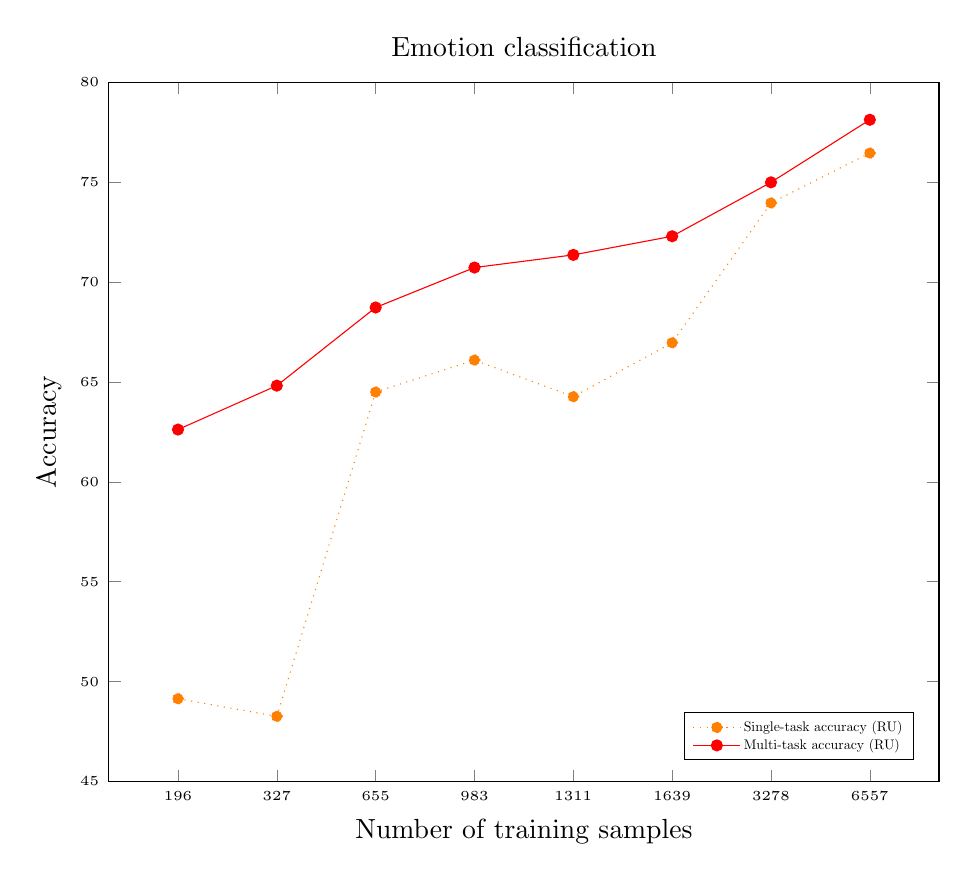
\begin{tikzpicture}[scale=1]
\begin{axis}[xlabel = Number of training samples,
ylabel = Accuracy,
title=Emotion classification,
legend pos= south east,
width=\textwidth,
% width=10cm,
% height=10cm,
% xmin=2,
% xmax=100,
xtick={0,1,2,3,4,5,6,7},
xticklabels={196, 327, 655, 983, 1311, 1639, 3278, 6557},
ymin=45,ymax=80,
legend cell align={left},
legend style={nodes={scale=0.5, transform shape}}
]
\addplot[color=orange,dotted, mark=*] coordinates {
(0, 49.14)
(1, 48.260000000000005)
(2, 64.5)
(3, 66.10000000000001)
(4, 64.26666666666667)
(5, 66.96666666666665)
(6, 73.96666666666667)
(7, 76.46666666666667)
};
\addlegendentry{Single-task accuracy (RU)}
\addplot[color=red,solid,mark=*] coordinates {
(0, 62.61999999999999)
(1, 64.82000000000001)
(2, 68.73333333333333)
(3, 70.73333333333333)
(4, 71.36666666666667)
(5, 72.3)
(6, 75.0)
(7, 78.13333333333334)};
\addlegendentry{Multi-task accuracy (RU)}
\end{axis}%
\end{tikzpicture}
\end{subfigure}
\end{figure}
\end{frame}

\begin{frame}{Encoder-agnostic models: the effect of training sample reduction by task}
\pgfplotsset{every tick label/.append style={font=\tiny}}
\begin{figure}
\begin{subfigure}{0.48\textwidth}
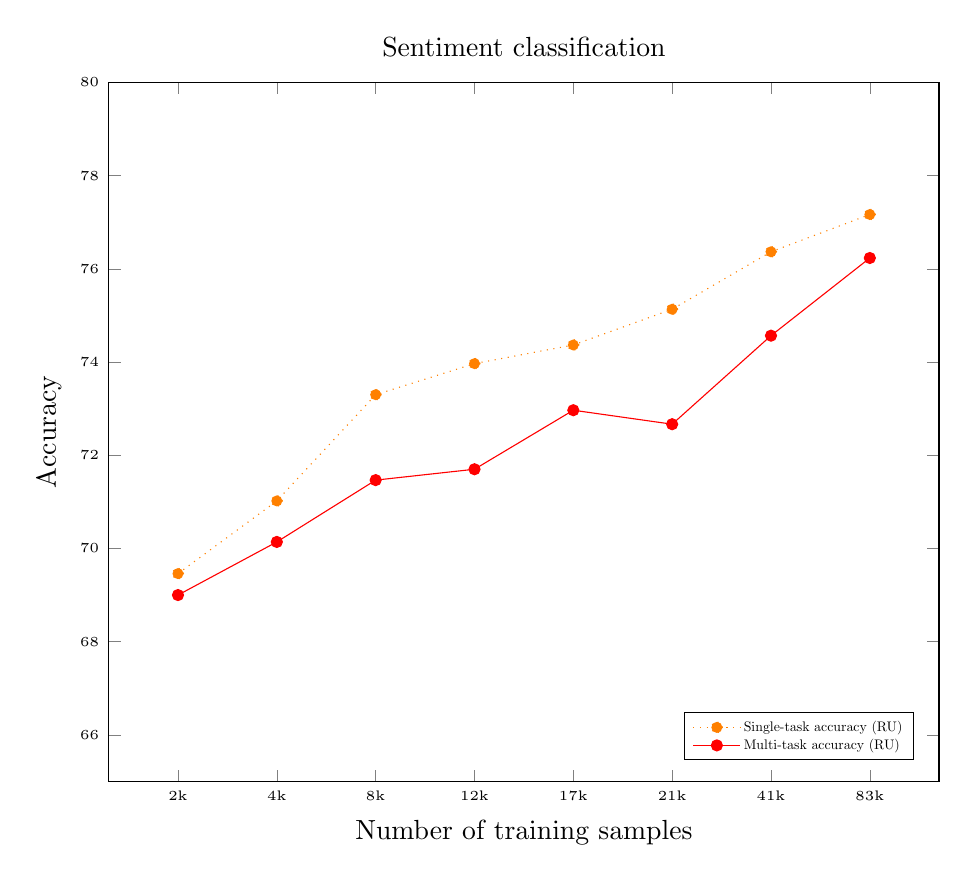
\begin{tikzpicture}[scale=1]
\begin{axis}[xlabel = Number of training samples,
ylabel = Accuracy,
title=Sentiment classification,
legend pos= south east,
width=\textwidth,
% width=10cm,
% height=10cm,
% xmin=2,
% xmax=100,
xtick={0,1,2,3,4,5,6,7},
xticklabels={2k, 4k, 8k, 12k, 17k, 21k, 41k, 83k},
ymin=65,ymax=80,
legend cell align={left},
legend style={nodes={scale=0.5, transform shape}}
]
\addplot[color=orange,dotted, mark=*] coordinates {
(0, 69.46000000000001)
(1, 71.02000000000001)
(2, 73.3)
(3, 73.96666666666665)
(4, 74.36666666666666)
(5, 75.13333333333334)
(6, 76.36666666666667)
(7, 77.16666666666667)
};
\addlegendentry{Single-task accuracy (RU)}
\addplot[color=red,solid,mark=*] coordinates {
(0, 68.99999999999999)
(1, 70.14)
(2, 71.46666666666665)
(3, 71.7)
(4, 72.96666666666667)
(5, 72.66666666666667)
(6, 74.56666666666666)
(7, 76.23333333333333)};
\addlegendentry{Multi-task accuracy (RU)}
\end{axis}%
\end{tikzpicture}
\end{subfigure}
\begin{subfigure}{0.48\textwidth}
\begin{tikzpicture}[scale=1]
\begin{axis}[xlabel = Number of training samples,
ylabel = Accuracy,
title=Toxicity classification,
legend pos= south east,
width=\textwidth,
% width=10cm,
% height=10cm,
% xmin=2,
% xmax=100,
xtick={0,1,2,3,4,5,6,7},
xticklabels={3k, 5k, 9k, 14k, 19k, 23k, 47k, 93k},
ymin=90,ymax=100,
legend cell align={left},
legend style={nodes={scale=0.5, transform shape}}
]
\addplot[color=orange,dotted, mark=*] coordinates {
(0, 91.50000000000001)
(1, 92.70000000000002)
(2, 93.93333333333334)
(3, 94.80000000000001)
(4, 95.06666666666666)
(5, 95.36666666666667)
(6, 96.13333333333333)
(7, 96.7)
};
\addlegendentry{Single-task accuracy (RU)}
\addplot[color=red,solid,mark=*] coordinates {
(0, 91.24000000000001)
(1, 92.6)
(2, 93.96666666666665)
(3, 94.60000000000001)
(4, 95.0)
(5, 95.33333333333333)
(6, 96.0)
(7, 96.5)};
\addlegendentry{Multi-task accuracy (RU)}
\end{axis}%
\end{tikzpicture}
\end{subfigure}
\end{figure}
\end{frame}

\begin{frame}{Encoder-agnostic models: the effect of training sample reduction by task}
\pgfplotsset{every tick label/.append style={font=\tiny}}
\begin{figure}
\begin{subfigure}{0.48\textwidth}
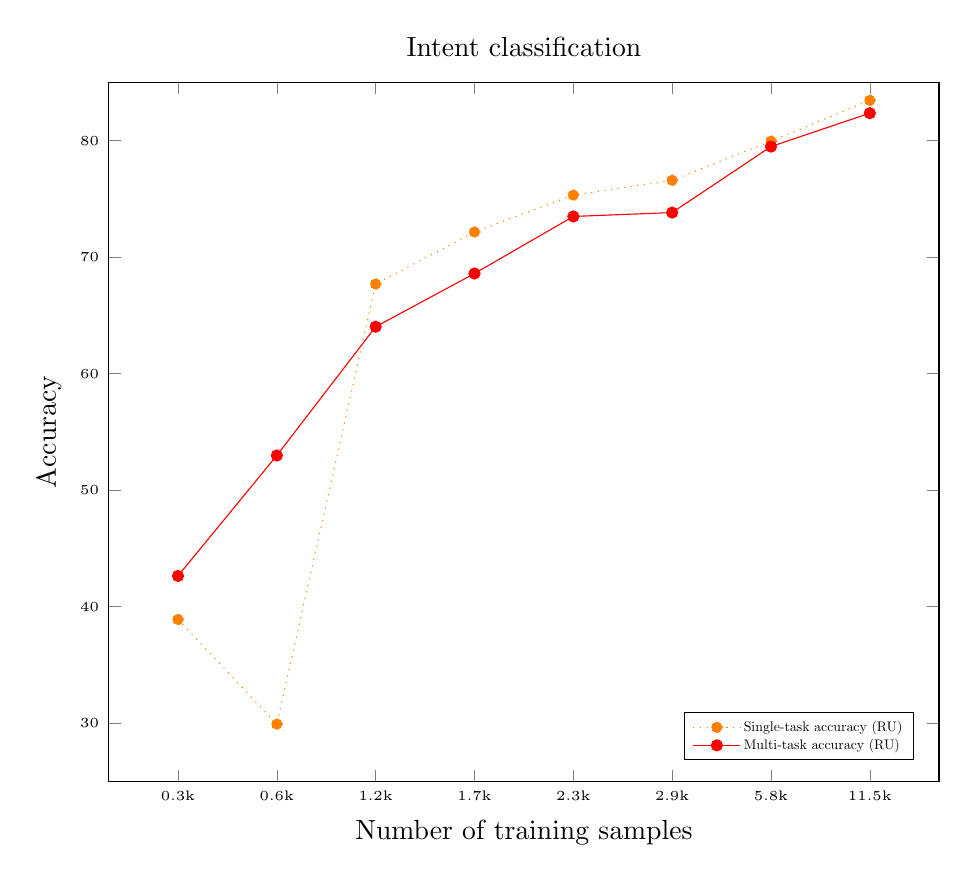
\begin{tikzpicture}
\begin{axis}[xlabel = Number of training samples,
ylabel = Accuracy,
title=Intent classification,
legend pos= south east,
width=\textwidth,
% width=10cm,
% height=10cm,
% xmin=2,
% xmax=100,
xtick={0,1,2,3,4,5,6,7},
xticklabels={0.3k, 0.6k, 1.2k, 1.7k, 2.3k, 2.9k, 5.8k, 11.5k},
ymin=25,ymax=85,
legend cell align={left},
legend style={nodes={scale=0.5, transform shape}}
]
\addplot[color=orange,dotted, mark=*] coordinates {
(0, 38.9)
(1, 29.920000000000005)
(2, 67.7)
(3, 72.16666666666667)
(4, 75.33333333333333)
(5, 76.60000000000001)
(6, 79.96666666666668)
(7, 83.46666666666665)
};
\addlegendentry{Single-task accuracy (RU)}
\addplot[color=red,solid,mark=*] coordinates {
(0, 42.64)
(1, 52.98)
(2, 64.03333333333335)
(3, 68.6)
(4, 73.5)
(5, 73.83333333333333)
(6, 79.5)
(7, 82.36666666666667)};
\addlegendentry{Multi-task accuracy (RU)}
\end{axis}
\end{tikzpicture}
\end{subfigure}
\begin{subfigure}{0.48\textwidth}
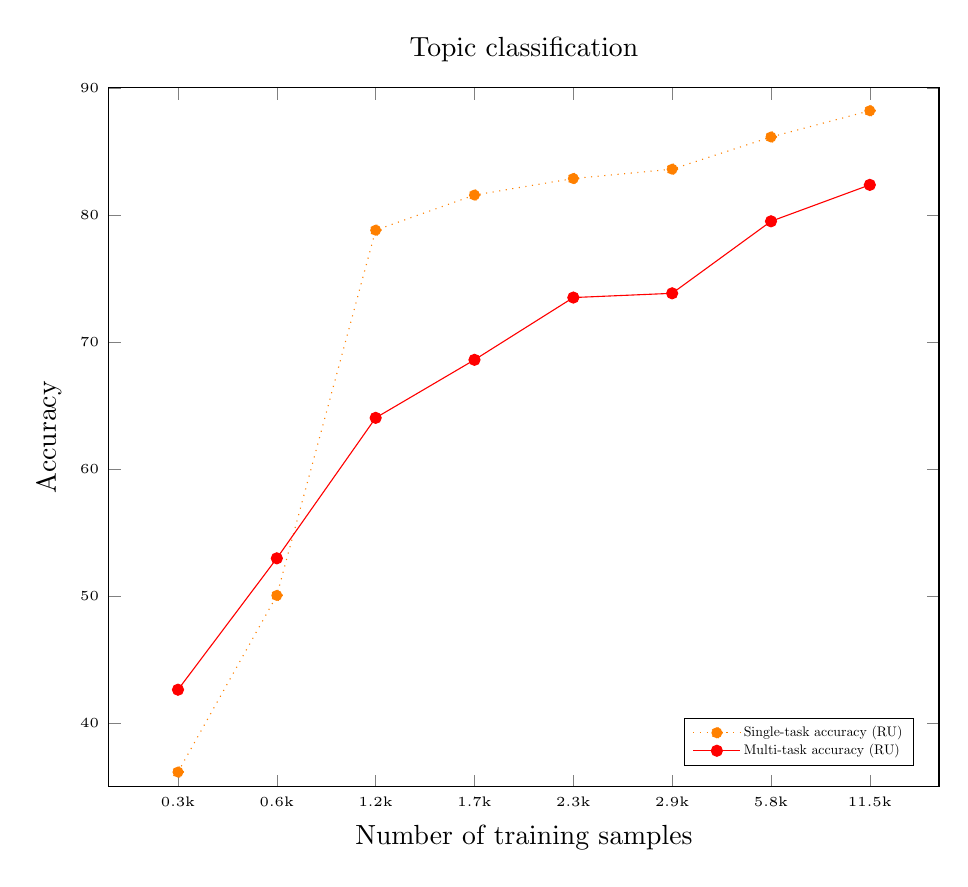
\begin{tikzpicture}
\begin{axis}[xlabel = Number of training samples,
ylabel = Accuracy,
title=Topic classification,
legend pos= south east,
width=\textwidth,
% width=10cm,
% height=10cm,
% xmin=2,
% xmax=100,
xtick={0,1,2,3,4,5,6,7},
xticklabels={0.3k, 0.6k, 1.2k, 1.7k, 2.3k, 2.9k, 5.8k, 11.5k},
ymin=35,ymax=90,
legend cell align={left},
legend style={nodes={scale=0.5, transform shape}}
]
\addplot[color=orange,dotted, mark=*] coordinates {
(0, 36.16)
(1, 50.06)
(2, 78.80000000000001)
(3, 81.56666666666666)
(4, 82.86666666666666)
(5, 83.60000000000001)
(6, 86.13333333333334)
(7, 88.2)
};
\addlegendentry{Single-task accuracy (RU)}
\addplot[color=red,solid,mark=*] coordinates {
(0, 42.64)
(1, 52.98)
(2, 64.03333333333335)
(3, 68.6)
(4, 73.5)
(5, 73.83333333333333)
(6, 79.5)
(7, 82.36666666666667)};
\addlegendentry{Multi-task accuracy (RU)}
\end{axis}%
\end{tikzpicture}
\end{subfigure}
\end{figure}
\end{frame}

\begin{frame}{Encoder-agnostic models: conclusions}
\begin{enumerate}
\item Многозадачные энкодер-агностичные модели - почти как однозадачные. Если для какой-то задачи данных мало, но для другой похожей задачи их много - то даже лучше.
\item Если данных становится очень мало, то многозадачные модели становятся сильно лучше однозадачных. Опять же, зависит от размера данных для задачи.
\item Добавление английских данных к русским - улучшает метрики многоязычных моделей, чем меньше русских данных - тем сильнее (до нескольких процентов). Это верно и для однозадачных моделей, при любом языке валидации.
\end{enumerate}
\end{frame}

\begin{frame}{Спасибо за внимание}
\end{frame}
